% Milestone 2 report -- CRAN Polish Mirror Demand & GitHub Release Pulse Analysis System
% Build: latexmk -pdf Milestone_2.tex     (output to be renamed TeamName_Report.pdf)
\documentclass[11pt,a4paper]{article}

\usepackage[utf8]{inputenc}
\usepackage[T1]{fontenc}
\usepackage{lmodern}
\usepackage[margin=2.3cm]{geometry}
\usepackage{graphicx}
\usepackage{booktabs}
\usepackage{tabularx}
\usepackage{longtable}
\usepackage{array}
\usepackage{multirow}
\usepackage{enumitem}
\usepackage{xcolor}
\usepackage{float}
\usepackage[font=small,labelfont=bf]{caption}
\usepackage{listings}
\usepackage{fancyhdr}
\usepackage{tikz}
\usetikzlibrary{arrows.meta,positioning,fit,backgrounds,calc}
\usepackage[colorlinks=true,linkcolor=blue!50!black,urlcolor=blue!50!black]{hyperref}

\setlist{itemsep=2pt,topsep=4pt}
\usepackage{ragged2e}
\usepackage{needspace}
\emergencystretch=3em
\setcounter{tocdepth}{1}
\newcolumntype{L}[1]{>{\RaggedRight\arraybackslash}p{#1}}
\newcolumntype{Y}{>{\RaggedRight\arraybackslash}X}
\newcommand{\hd}[1]{\par\Needspace{7\baselineskip}\medskip\noindent\textbf{#1}\par\nopagebreak\smallskip}
\captionsetup[table]{position=top,skip=4pt}
\setlength{\parindent}{0pt}
\setlength{\parskip}{5pt}
\renewcommand{\arraystretch}{1.15}

\pagestyle{fancy}
\fancyhf{}
\lhead{Big Data Analysis Classes | 2026Z}
\rhead{Milestone 2 -- Project Report}
\cfoot{\thepage}

% Team name is not fixed in the repo: change it here (also used for the output PDF name).
\newcommand{\teamname}{TeamName}

% Visible marker for facts that must still be filled in or verified before submission.
\newcommand{\todo}[1]{\textcolor{red}{\textbf{[TODO: #1]}}}
% Status markers used in the architecture and technology tables.
\newcommand{\done}{\textbf{Implemented}}
\newcommand{\planned}{\textit{Work in progress}}
\newcommand{\partialimpl}{\textit{Partial}}

\lstset{basicstyle=\ttfamily\footnotesize,breaklines=true,frame=single,columns=fullflexible,
  keepspaces=true,showstringspaces=false}

\title{\textbf{Project: CRAN Polish Mirror Demand \& GitHub Release Pulse Analysis System}\\[4pt]
\large Milestone 2 -- Project Report}
\author{Jakub Grzywaczewski, Mateusz Nizwantowski, Aleks Kapich, \L{}ukasz Grabarski}
\date{\today}

\begin{document}
\maketitle
\tableofcontents
\newpage

% =====================================================================
\section{Updates to the Milestone 1 Report}
% =====================================================================

This section lists every assumption of Milestone 1 (PM1) that changed during implementation, with the
reason. Everything not listed here (project description, purpose, users, deliverables, business process,
team allocation) is unchanged and kept in Section~\ref{sec:pm1}.

\subsection{Business assumptions}

\begin{itemize}
  \item \textbf{No change} to purpose, target users, the three user-facing deliverables (real-time demand
        dashboard, version adoption and lag analytics, mirror health view) or the two business cases
        (load forecasting, bot detection).
  \item \todo{Confirm with the team whether any business case or deliverable was dropped or re-scoped.}
\end{itemize}

\subsection{Technical assumptions}

{\footnotesize
\begin{longtable}{@{}L{2.0cm}L{2.7cm}L{4.7cm}L{5.0cm}@{}}
\caption{Changes with respect to Milestone 1.}\\
\toprule
\textbf{Topic} & \textbf{PM1 assumption} & \textbf{Now} & \textbf{Justification} \\
\midrule
\endfirsthead
\toprule
\textbf{Topic} & \textbf{PM1 assumption} & \textbf{Now} & \textbf{Justification} \\
\midrule
\endhead
\bottomrule
\endfoot
Kafka topics &
  \texttt{cran.downloads}, \texttt{gh.events.raw} (JSON) &
  \texttt{cran\_\allowbreak{}mirror\_\allowbreak{}logs}, \texttt{cran\_\allowbreak{}mirror\_\allowbreak{}logs\_\allowbreak{}clean}, \texttt{cran\_\allowbreak{}mirror\_\allowbreak{}package\_\allowbreak{}downloads},
  \texttt{github\_\allowbreak{}repo\_\allowbreak{}updates}, \texttt{github\_\allowbreak{}repo\_\allowbreak{}updates\_\allowbreak{}clean}, \texttt{github\_\allowbreak{}repo\_\allowbreak{}list} &
  Raw, validated and derived data are separated into distinct topics (a raw topic is never overwritten),
  which also makes reprocessing and quality checks possible. Dots in topic names were avoided
  (Kafka warns about collisions between \texttt{.} and \texttt{\_\allowbreak{}}). Topics have 3 partitions and are keyed
  (\texttt{package\_\allowbreak{}name}, \texttt{repo\_\allowbreak{}name}), so all records of one package or repository stay
  ordered in one partition. \\
Message format &
  JSON &
  Raw: text (log line) / JSON (GitHub). Clean: \textbf{Avro} with Confluent Schema Registry &
  Avro gives enforced, versioned, backward-compatible schemas and compact messages. A job refuses to
  start if its columns drift from the \texttt{.avsc} file. \\
CRAN log source &
  Python daemon tailing the live log file, syslog &
  \textbf{Filebeat} installed on the original mirror tails the access log and produces each line to Kafka (work in progress). Until then a \textbf{log generator} simulates the stream in dev &
  Filebeat is a lightweight, proven shipper for file tailing with built-in Kafka output, offsets and retries, so no custom daemon has to be maintained on the mirror. \\
Log format &
  W3C/Nginx log with User-Agent; bot filtering by User-Agent &
  Apache \emph{common} log format (no referrer, no User-Agent) &
  The mirror's logs contain only IP, time, request, status and size. Bot and CI detection therefore
  cannot use the User-Agent and must rely on per-client behaviour (request rate, 404 ratio, path
  patterns); this is why the bot business case is modelled as sessions classification. \\
Late and invalid data &
  Event-time watermark with 30\,s allowed lateness &
  Ingest jobs reject records more than 5\,min in the future or more than 7 days in the past (relative to Kafka arrival time), with a
  \texttt{reject\_\allowbreak{}reason}. The 30\,s watermark stays the plan for the windowed jobs (work in progress) &
  A watermark only helps windowed aggregations, which are not built yet. The ingest rule protects the Parquet sink (one open writer per
  event hour) from unbounded history, e.g.\ the 90 days returned on the first poll of a GitHub timeline. Rejected records are kept, not lost. \\
Non-download requests &
  Ingestion discards non-artifact GET requests &
  All parseable requests are kept in \texttt{cran\_\allowbreak{}mirror\_\allowbreak{}logs\_\allowbreak{}clean}; only the downloads job keeps package files &
  Bot detection needs the full request history of a client (paths, 404 ratio, non-package requests), which a download-only stream would lose.
  Filtering is therefore done in a derived topic, not at ingestion. \\
Raw and clean storage &
  Kafka appended to HDFS as Parquet &
  Flink writes raw lines unchanged as text and validated records as Parquet (Snappy); files are finalised on checkpoint (60\,s) &
  Raw data is kept byte for byte, so it can be re-parsed if rules change. Only typed, validated data is Parquet. The same Flink job
  does both writes, so no separate consumer or connector has to be run, and readers never see half-written files. \\
GitHub acquisition &
  Poller with ETag, 5\,000 req/h limit &
  Two-tier watch-list poller (tier~1 every 120\,s, tier~2 within a 3\,500 req/h budget), org timelines
  instead of per-repo polling, SQLite state, optional global feed &
  Staying inside the quota for $\sim$18\,000 packages required prioritisation and a request budget
  (see Section~\ref{sec:acq}). \\
Cluster topology &
  Distributed, fault-tolerant services (implied) &
  One VM per environment; single-node Kafka, Schema Registry, Cassandra and Flink (1 TaskManager, 7 slots); HDFS with 3 DataNodes and replication 2 &
  Infrastructure is one VM each for stage and prod, so services run as single containers. Kafka and Cassandra use replication factor~1.
  The software and data flow are the same as in a cluster, so scaling out later needs configuration changes, not a redesign. \\
GeoIP enrichment &
  Client IP enriched with country and city (PM1 Figure~2) &
  Not implemented; the client IP is kept as is &
  \todo{Confirm the reason (e.g.\ the mirror is Polish, so location adds little) and whether it stays out of scope.} \\
Airflow &
  Daily DAGs pulling crantogit, PySpark, Cassandra refresh &
  Airflow 3 running; only a connectivity-check DAG exists &
  Platform work first; production DAGs follow the Spark jobs (see Section~\ref{sec:analytics}). \\
Batch storage &
  HDFS/Parquet by source and date &
  Parquet partitioned \texttt{dt=YYYY-MM-DD/hr=HH}; \texttt{raw}, \texttt{clean} and \texttt{raw\_\allowbreak{}bad} zones &
  Hourly partitions suit hourly forecasting; the extra \emph{bad} zone preserves rejected records. \\
\end{longtable}}

\subsection{Implementation status}

\begin{table}[H]
\centering
\caption{Implementation status at Milestone 2.}
\small
\begin{tabularx}{\textwidth}{@{}L{4.3cm}L{1.3cm}L{3.0cm}Y@{}}
\toprule
\textbf{Component} & \textbf{Version} & \textbf{Status} & \textbf{Comment} \\
\midrule
Kafka (KRaft) & 4.3.2 & \done & 6 data topics, 3 partitions, RF~1 \\
Schema Registry (Confluent) & 8.4.1 & \done & 3 Avro subjects \\
PyFlink & 1.20.3 & \partialimpl & 3 ingest/validation jobs; windowed aggregations, joins and inference \planned \\
HDFS & 3.4.2 & \done & 1 DataNode (dev), 3 DataNodes with replication 2 (stage/prod) \\
Cassandra & 5.0.9 & \partialimpl & Keyspace \texttt{cran\_\allowbreak{}analytics} exists; \texttt{rt\_\allowbreak{}*}/\texttt{batch\_\allowbreak{}*} tables \planned \\
Airflow & 3.4.0 & \partialimpl & Running, logs on HDFS; production DAGs \planned \\
GitHub poller & -- & \done & Python, with unit tests \\
PySpark & -- & \planned & Batch aggregates, features, training \\
MLflow & -- & \planned & Tracking and model registry \\
Streamlit & -- & \planned & Dashboard \\
\bottomrule
\end{tabularx}
\end{table}

% =====================================================================
\section{Conceptual Data Model}
% =====================================================================

\subsection{Key entities and relationships}

\begin{itemize}
  \item \textbf{Package} -- an R package on CRAN (name). Key of the model.
  \item \textbf{Repository} -- the upstream GitHub repository (\texttt{owner/repo}, \texttt{repo\_\allowbreak{}id}).
        \emph{Package} $N$--$1$ \emph{Repository}: a repository can hold several CRAN packages (mapping from crantogit);
        $\sim$10--15\% of packages have no GitHub repository.
  \item \textbf{GitHubEvent} -- an event on a repository (\texttt{ReleaseEvent}, \texttt{PushEvent}, \texttt{CreateEvent}, \ldots).
        \emph{Repository} $1$--$N$ \emph{GitHubEvent}. A \texttt{ReleaseEvent}/tag event carries the release tag.
  \item \textbf{Release} -- a version of a package (\texttt{package\_\allowbreak{}name}, \texttt{version}); a derived entity
        linking a GitHub tag with a CRAN artifact.
  \item \textbf{Download} -- one successful or failed fetch of a package artifact from the mirror.
        \emph{Package} $1$--$N$ \emph{Download}; \emph{Release} $1$--$N$ \emph{Download}.
  \item \textbf{Client} -- an IP address; \emph{Client} $1$--$N$ \emph{Download} (basis for bot detection).
  \item \textbf{WatchlistEntry} -- a row of the poller's watch-list (\texttt{package}, \texttt{owner}, \texttt{repo},
        \texttt{endpoint}, \texttt{tier}); defines which repositories are observed.
\end{itemize}

\begin{figure}[H]
\centering
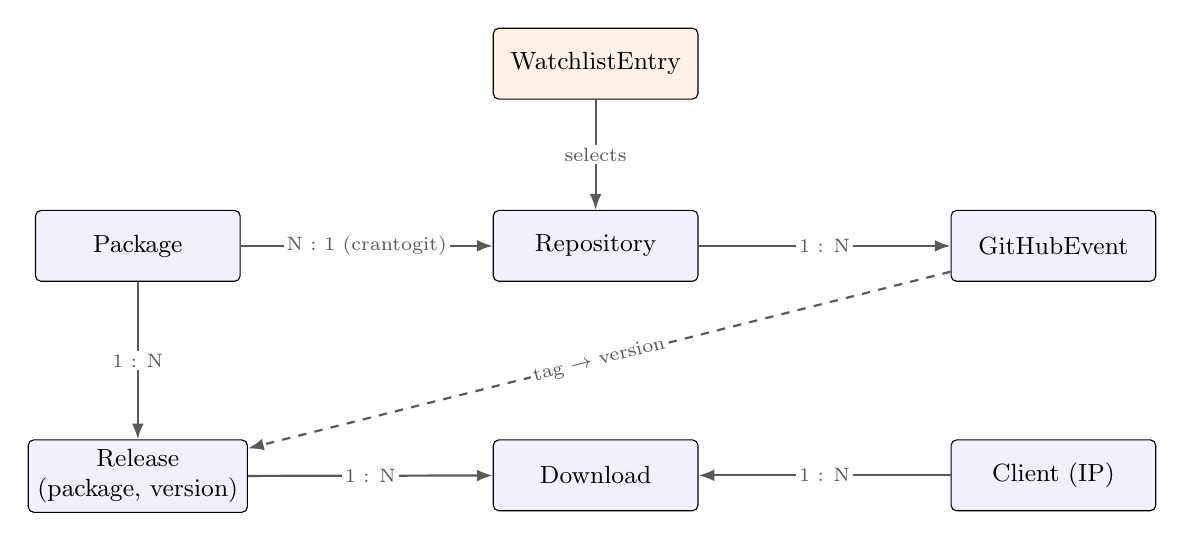
\begin{tikzpicture}[
  ent/.style={draw,rounded corners=2pt,minimum width=2.6cm,minimum height=0.9cm,align=center,fill=blue!6,font=\small},
  rel/.style={-{Latex[length=2mm]},thick,gray!70!black},
  lab/.style={font=\scriptsize,fill=white,inner sep=1pt}]
  \node[ent] (pkg) {Package};
  \node[ent,right=3.2cm of pkg] (repo) {Repository};
  \node[ent,right=3.2cm of repo] (ev) {GitHubEvent};
  \node[ent,below=2cm of pkg] (rel) {Release\\(package, version)};
  \node[ent,below=2cm of repo] (dl) {Download};
  \node[ent,below=2cm of ev] (cl) {Client (IP)};
  \node[ent,above=1.4cm of repo,fill=orange!10] (wl) {WatchlistEntry};
  \draw[rel] (pkg) -- node[lab]{N : 1 (crantogit)} (repo);
  \draw[rel] (repo) -- node[lab]{1 : N} (ev);
  \draw[rel] (pkg) -- node[lab]{1 : N} (rel);
  \draw[rel] (rel) -- node[lab]{1 : N} (dl);
  \draw[rel] (cl) -- node[lab]{1 : N} (dl);
  \draw[rel] (wl) -- node[lab,pos=0.5]{selects} (repo);
  \draw[rel,dashed] (ev) -- node[lab,sloped]{tag $\to$ version} (rel);
\end{tikzpicture}
\caption{Conceptual data model: entities and relationships.}
\label{fig:erd}
\end{figure}

\subsection{Description of data sets}

\begin{table}[H]
\centering
\caption{Data sets used in the project.}
\scriptsize
\begin{tabularx}{\textwidth}{@{}L{2.0cm}YYY@{}}
\toprule
 & \textbf{A. CRAN mirror access logs} & \textbf{B. GitHub Events} & \textbf{C. crantogit mapping} \\
\midrule
Category & Web server access log: package downloads from the Polish mirror (cran.mi2.ai) &
  Software development activity on repositories behind CRAN packages &
  Reference data: CRAN package $\to$ GitHub repository \\
Source format & Apache common log, plain text &
  JSON (GitHub REST API, \texttt{/events}, \texttt{/orgs/\{o\}/events}, \texttt{/repos/\{o\}/\{r\}/events}) &
  CSV \\
Inflow & Stream, $\sim$2--4 req/s (PM1 estimate; $\sim$7\,400 lines per hour in the sample file) \todo{measure on production logs} &
  Stream by polling; volume depends on watch-list size \todo{measure events/hour from the poller run report} &
  Batch, one daily pull \\
Avg.\ records & $\sim$170\,000--350\,000 lines/day \todo{verify} &
  \todo{events/day} &
  $\sim$18\,000 rows \\
Size & $\sim$500--700\,MB/month & $\sim$50--100\,MB/month & $\sim$1\,MB \\
Time period & From the start of collection; history from the mirror \todo{state exact period} &
  Live from the start of polling; first poll of a timeline returns up to 90 days (limited to 7 days by the Flink validation) &
  Current snapshot, refreshed daily \\
Features & Client IP, timestamp, HTTP method, path, protocol, status, bytes sent &
  Event id/type, \texttt{created\_\allowbreak{}at}, repo id/name, actor id/login, organisation, ref, ref type, release tag, payload &
  Package name, GitHub owner, repository URL, \ldots \\
\bottomrule
\end{tabularx}
\end{table}

\subsubsection{Record layouts}

\hd{A1. Raw log line} (topic \texttt{cran\_\allowbreak{}mirror\_\allowbreak{}logs}; one string per message)
\begin{lstlisting}
23.21.250.48 - - [15/Oct/2026:14:06:45 +0000] "GET /src/contrib/Archive/DescTools/DescTools_0.99.14.tar.gz HTTP/1.1" 200 2009727
\end{lstlisting}

\begin{figure}[H]
\centering
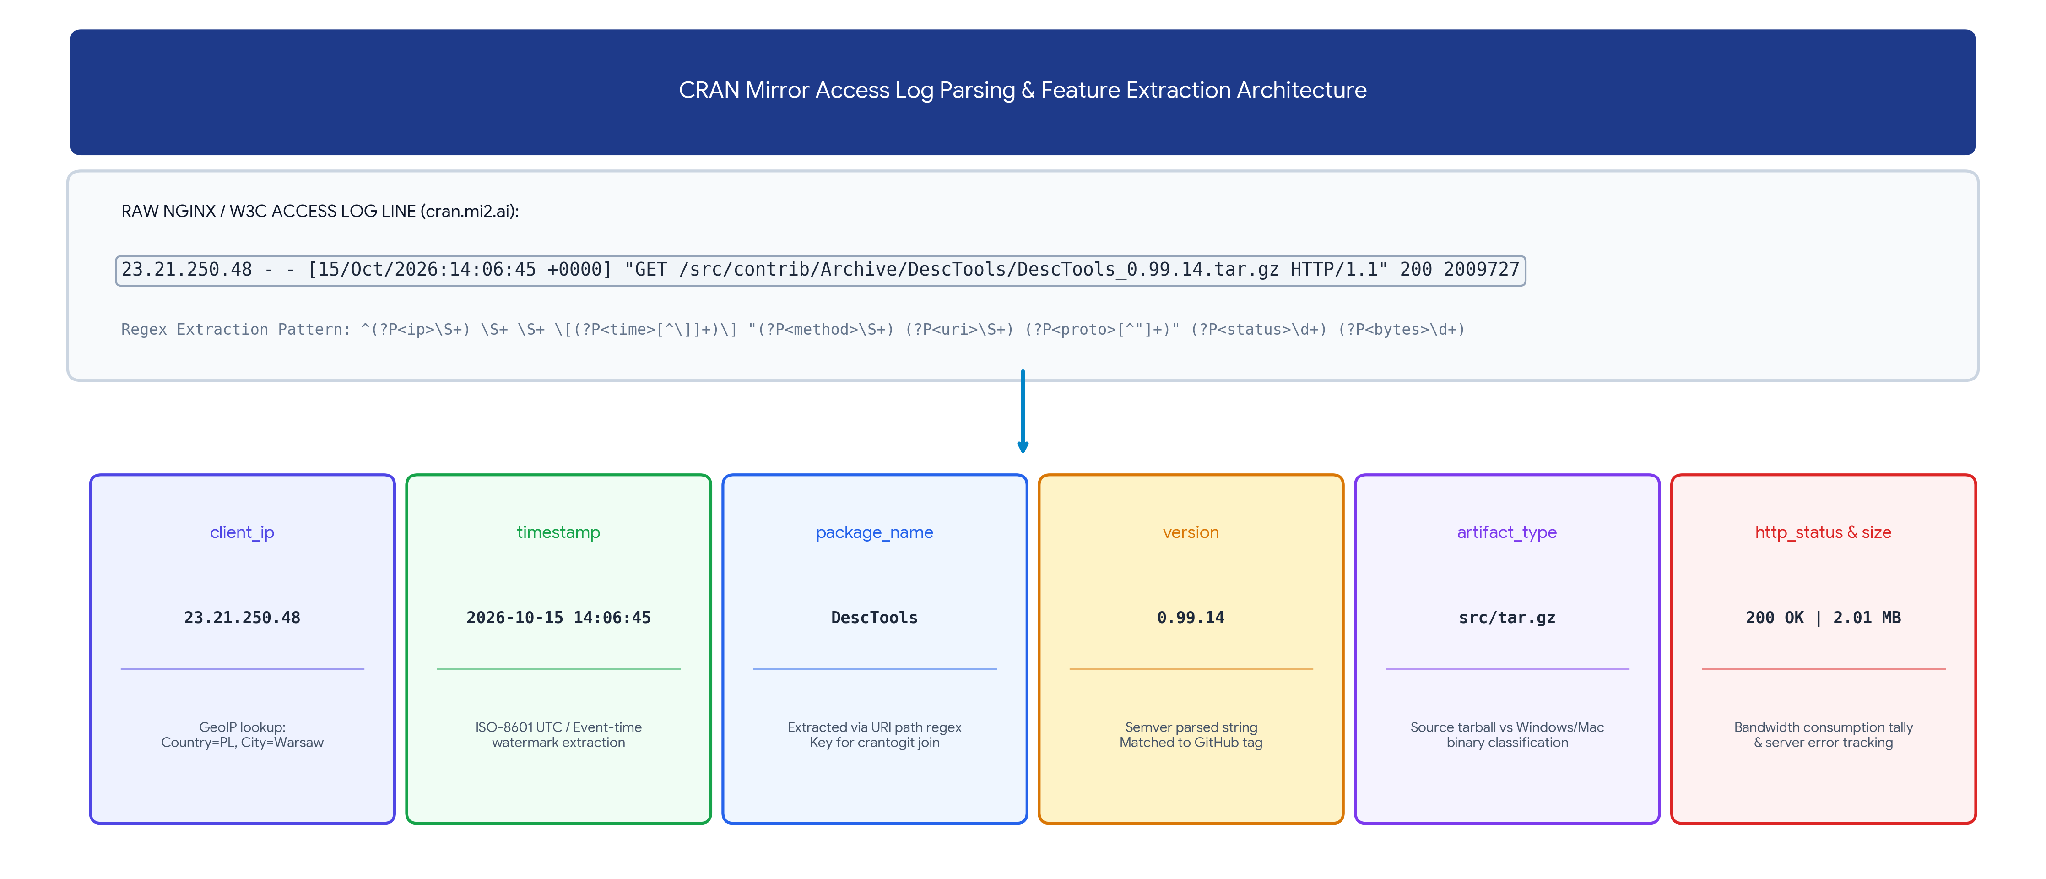
\includegraphics[width=\textwidth]{figures/fig_log_parsing.png}
\caption{Parsing of a raw log line into attributes (from Milestone 1). The implemented pipeline uses the
common log format without User-Agent, and no GeoIP enrichment.}
\end{figure}

\hd{A2. Clean log record} (\texttt{cran\_\allowbreak{}mirror\_\allowbreak{}logs\_\allowbreak{}clean}, Avro \texttt{CranMirrorLogClean})

\begin{center}
\centering\small
\begin{tabularx}{\textwidth}{@{}llY@{}}
\toprule
\textbf{Field} & \textbf{Type} & \textbf{Meaning} \\
\midrule
\texttt{event\_\allowbreak{}ts} & timestamp-millis & Request time from the log line (UTC) \\
\texttt{arrival\_\allowbreak{}ts} & timestamp-millis & Time the line arrived in Kafka \\
\texttt{ip} & string & Client address (IPv4/IPv6) \\
\texttt{http\_\allowbreak{}method} & string & HTTP method, upper case \\
\texttt{path} & string & Requested path with query string \\
\texttt{protocol} & string & e.g.\ HTTP/1.1 \\
\texttt{status} & int & HTTP status (100--599) \\
\texttt{bytes\_\allowbreak{}sent} & long, nullable & Response size; null when the log has \texttt{-} \\
\bottomrule
\end{tabularx}
\end{center}

\hd{A3. Package download record} (\texttt{cran\_\allowbreak{}mirror\_\allowbreak{}package\_\allowbreak{}downloads}, Avro \texttt{CranMirrorPackageDownload}, key \texttt{package\_\allowbreak{}name})

\begin{center}
\centering\small
\begin{tabularx}{\textwidth}{@{}llY@{}}
\toprule
\textbf{Field} & \textbf{Type} & \textbf{Meaning} \\
\midrule
\texttt{event\_\allowbreak{}ts}, \texttt{arrival\_\allowbreak{}ts}, \texttt{ip}, \texttt{http\_\allowbreak{}method} & as in A2 & carried over \\
\texttt{package\_\allowbreak{}name} & string & From the file name, e.g.\ \texttt{Ckmeans.1d.dp} \\
\texttt{package\_\allowbreak{}version} & string & From the file name, e.g.\ \texttt{0.0.2-6} \\
\texttt{artifact\_\allowbreak{}type} & string & \texttt{tar.gz}, \texttt{tgz}, \texttt{zip} \\
\texttt{target\_\allowbreak{}system} & string & \texttt{source}, \texttt{macos}, \texttt{windows} \\
\texttt{outcome} & string & \texttt{SUCCESS} (status $<400$) or \texttt{FAILURE} \\
\bottomrule
\end{tabularx}
\end{center}

\hd{B. GitHub event record} (\texttt{github\_\allowbreak{}repo\_\allowbreak{}updates\_\allowbreak{}clean}, Avro \texttt{GithubRepoUpdateClean}, key \texttt{repo\_\allowbreak{}name})

\begin{center}
\centering\small
\begin{tabularx}{\textwidth}{@{}llY@{}}
\toprule
\textbf{Field} & \textbf{Type} & \textbf{Meaning} \\
\midrule
\texttt{event\_\allowbreak{}id} & string & GitHub event id (deduplication key, 48\,h state) \\
\texttt{event\_\allowbreak{}type} & string & \texttt{PushEvent}, \texttt{ReleaseEvent}, \texttt{CreateEvent}, \ldots \\
\texttt{event\_\allowbreak{}ts} & timestamp-millis & GitHub's \texttt{created\_\allowbreak{}at} (event time) \\
\texttt{fetched\_\allowbreak{}ts} & timestamp-millis & When the poller received the event \\
\texttt{track} & string & \texttt{global} or \texttt{watchlist} \\
\texttt{endpoint} & string & Timeline the event was read from \\
\texttt{repo\_\allowbreak{}id}, \texttt{repo\_\allowbreak{}name} & long, string & Repository \\
\texttt{actor\_\allowbreak{}id}, \texttt{actor\_\allowbreak{}login} & long, string & Acting user \\
\texttt{org\_\allowbreak{}login} & string, nullable & Owning organisation \\
\texttt{packages} & array<string> & CRAN packages in the repository (from watch-list) \\
\texttt{ref}, \texttt{ref\_\allowbreak{}type} & string, nullable & Branch/tag reference \\
\texttt{release\_\allowbreak{}tag} & string, nullable & \texttt{payload.release.tag\_\allowbreak{}name} \\
\texttt{payload\_\allowbreak{}json} & string & Original payload as JSON \\
\bottomrule
\end{tabularx}
\end{center}

\hd{C. crantogit mapping and watch-list} The poller turns \texttt{crantogit.csv} into
\texttt{watchlist.csv} (\texttt{package, owner, repo, endpoint, tier}); each row is also published to
\texttt{github\_\allowbreak{}repo\_\allowbreak{}list} as JSON.

\subsection{Data quality assessment}

\begin{table}[H]
\centering
\caption{Data quality assessment.}
\small
\begin{tabularx}{\textwidth}{@{}L{2.6cm}Y@{}}
\toprule
\textbf{Source} & \textbf{Assessment} \\
\midrule
CRAN logs &
  Highly regular format. Issues: requests that are not package downloads (HTML pages, \texttt{PACKAGES.rds}, check results)
  -- removed by the download extraction job; bot, scanner and health-check traffic -- no User-Agent available;
  non-UTC offsets, future or very old timestamps -- rejected (\texttt{invalid\_\allowbreak{}status}, \texttt{invalid\_\allowbreak{}method},
  \texttt{future\_\allowbreak{}timestamp}, \texttt{stale\_\allowbreak{}timestamp}, \texttt{unparseable}); \texttt{-} as size -- stored as null.
  \todo{Report the reject rate on a real run.} \\
GitHub events &
  Duplicates (at-least-once delivery and overlapping poll pages) -- removed on \texttt{event\_\allowbreak{}id}; stale history on first poll --
  rejected as \texttt{stale\_\allowbreak{}timestamp}; \texttt{PublicEvent} has the repository's creation date as \texttt{created\_\allowbreak{}at},
  so it is excluded from delay measurements; timelines hold at most 300 events, so a busy organisation can
  hide older events (mitigated by polling only mostly-R organisations); the 5\,000 req/h quota limits coverage of tier~2.
  \todo{Report the number of events, duplicates and rejects from \texttt{scripts/check\_\allowbreak{}run.py}.} \\
crantogit &
  10--15\% of packages are not on GitHub; one repository can contain several packages; mapping may be outdated
  (renamed/moved repositories answer 404/410 -- the poller rechecks them after 7 days). \\
\bottomrule
\end{tabularx}
\end{table}

\subsection{Features for machine learning}

\hd{Business case A -- hourly load forecasting (regression).}
\begin{center}
\centering\small
\begin{tabularx}{\textwidth}{@{}L{3.2cm}Y@{}}
\toprule
\textbf{Dependent (target)} & Number of downloads (and/or bytes served) in hour $t+h$, $h \in [1,168]$ (7 days ahead). \\
\midrule
\textbf{Independent} &
  Downloads and bytes in the previous 1, 2, \ldots, 24, 168 hours (lags); rolling mean/std over 24\,h and 7\,d;
  hour of day, day of week, holiday flag; number of distinct clients; share of failed requests;
  number of GitHub release events in the previous hours/days for top packages; share of top-$k$ packages. \\
\midrule
\textbf{Transformations} &
  Hourly aggregation of \texttt{cran\_\allowbreak{}mirror\_\allowbreak{}package\_\allowbreak{}downloads}; imputation of empty hours with 0;
  cyclic encoding of hour/day; log transform of counts; time-based train/validation split (no shuffling). \\
\bottomrule
\end{tabularx}
\end{center}

\hd{Business case B -- bot / CI client detection (classification).}
\begin{center}
\centering\small
\begin{tabularx}{\textwidth}{@{}L{3.2cm}Y@{}}
\toprule
\textbf{Dependent (target)} & Client class (\texttt{human} / \texttt{bot}) for a client session. Labels: \todo{decide labelling -- heuristic rules (weak labels) or manual sample; no User-Agent available}. \\
\midrule
\textbf{Independent} &
  Requests per session and per minute; mean inter-request time; share of 404/4xx; number of distinct packages;
  share of source vs binary artifacts; share of non-package paths; bytes per request; session duration;
  share of requests to archived versions. \\
\midrule
\textbf{Transformations} &
  Sessionisation per IP (gap $>$ 30\,min starts a new session); aggregation of session features from
  \texttt{cran\_\allowbreak{}mirror\_\allowbreak{}logs\_\allowbreak{}clean} (full path is needed, hence the clean log topic rather than the downloads topic);
  scaling; class imbalance handling. \\
\bottomrule
\end{tabularx}
\end{center}

\hd{Business case C -- adoption lag (statistical analysis / regression).}
Dependent variable: lag between a release event (\texttt{event\_\allowbreak{}ts} of the tag) and the peak of downloads of that version.
Independent variables: package popularity before the release, release type (major/minor/patch from the version),
day of week. The join key is \texttt{package\_\allowbreak{}name} (from \texttt{packages} in GitHub events) with the version in the tag.

% =====================================================================
\section{Data Acquisition and Transformation}\label{sec:acq}
% =====================================================================

\subsection{Acquisition strategy}

\begin{table}[H]
\centering
\caption{Acquisition strategy.}
\small
\begin{tabularx}{\textwidth}{@{}L{2.6cm}L{4.2cm}Y@{}}
\toprule
\textbf{Source} & \textbf{Technology} & \textbf{Limitations and handling} \\
\midrule
CRAN logs &
  Target: Filebeat on the original mirror $\to$ Kafka \texttt{cran\_\allowbreak{}mirror\_\allowbreak{}logs} (work in progress). Now: Python log generator, about 4 events/s (dev) &
  The generator only simulates the stream (same common log format, same topic), so downstream jobs do not change when Filebeat replaces it. The raw line is kept unchanged. \\
GitHub Events &
  Python poller (\texttt{poller/gh\_\allowbreak{}poller}), \texttt{requests}-based, \texttt{confluent-kafka} producer, SQLite state &
  Authenticated limit 5\,000 req/h; timelines hold $\le$300 events and 90 days; \texttt{X-Poll-Interval} must be respected.
  Handled by: conditional requests (\texttt{ETag}/\texttt{If-None-Match}; a 304 costs no quota); org timelines instead
  of per-repo polling when R repositories are $\ge$50\% of an organisation's public repos; tier~1 (120\,s) before tier~2
  (budget 3\,500 paid requests/h; interval raised automatically); at most 10 parallel polls and 300 req/min;
  interval doubling below 1\,000 remaining requests; pause on 403/429 until reset; retries 2/4/8\,s on 5xx. \\
crantogit &
  HTTP download of \texttt{crantogit.csv}, watch-list build (\texttt{python -m gh\_\allowbreak{}poller.watchlist}) &
  Account types (organisation/user) are cached so an interrupted build resumes. Runs daily (Airflow DAG \planned). \\
\bottomrule
\end{tabularx}
\end{table}

\hd{Delivery guarantees.} The poller uses an idempotent Kafka producer with \texttt{acks=all}; an event counts as written
only after Kafka confirms it, otherwise polling pauses for 60\,s and the timeline is re-fetched. Delivery is therefore
\emph{at least once}; duplicates are removed downstream on \texttt{event\_\allowbreak{}id}. Events larger than the broker limit (1\,MB)
are logged and dropped.

\subsection{Transformation steps and storage}

\begin{enumerate}
  \item \textbf{Raw landing.} Every raw message is stored unchanged: Kafka topic (\texttt{cran\_\allowbreak{}mirror\_\allowbreak{}logs},
        \texttt{github\_\allowbreak{}repo\_\allowbreak{}updates}) and HDFS text files \texttt{/data/raw/\ldots/dt=/hr=} (by arrival time).
  \item \textbf{Parsing and validation} (Flink job \texttt{cran\_\allowbreak{}logs\_\allowbreak{}ingest.py}): regular expression for the common log
        format, validation of method and status range, event-time plausibility. Valid records go to
        \texttt{cran\_\allowbreak{}mirror\_\allowbreak{}logs\_\allowbreak{}clean} (Avro) and \texttt{/data/clean/cran\_\allowbreak{}mirror\_\allowbreak{}logs} (Parquet, Snappy, by event time); invalid
        ones with a \texttt{reject\_\allowbreak{}reason} to \texttt{/data/raw/cran\_\allowbreak{}mirror\_\allowbreak{}logs\_\allowbreak{}bad}.
  \item \textbf{Download extraction} (\texttt{cran\_\allowbreak{}package\_\allowbreak{}downloads.py}): keeps only requests for
        \texttt{<name>\_\allowbreak{}<version>.\{tar.gz,tgz,zip\}}; derives \texttt{package\_\allowbreak{}name}, \texttt{package\_\allowbreak{}version},
        \texttt{artifact\_\allowbreak{}type}, \texttt{target\_\allowbreak{}system}, \texttt{outcome}; drops path, protocol and size. Output topic is keyed by package name
        so all downloads of a package stay ordered in one partition.
  \item \textbf{GitHub events} (\texttt{github\_\allowbreak{}events\_\allowbreak{}ingest.py}): JSON field extraction, timestamp and track validation,
        deduplication on \texttt{event\_\allowbreak{}id} (state TTL 48\,h), schema-checked Avro output keyed by \texttt{repo\_\allowbreak{}name}, Parquet by event time,
        rejects to \texttt{/data/raw/github\_\allowbreak{}repo\_\allowbreak{}updates\_\allowbreak{}bad}. Watch-list rows are copied to \texttt{/data/raw/github\_\allowbreak{}repo\_\allowbreak{}list}.
  \item \textbf{Aggregation and enrichment} \planned: windowed counters in Flink (speed layer) and Spark jobs over Parquet
        (batch layer), join of downloads with release events via the watch-list, output to Cassandra.
\end{enumerate}

\begin{table}[H]
\centering
\caption{Storage strategy.}
\small
\begin{tabularx}{\textwidth}{@{}L{4.6cm}L{2.7cm}L{3.2cm}Y@{}}
\toprule
\textbf{Store} & \textbf{Technology} & \textbf{Format} & \textbf{Content} \\
\midrule
\texttt{cran\_\allowbreak{}mirror\_\allowbreak{}logs}, \texttt{github\_\allowbreak{}repo\_\allowbreak{}updates}, \texttt{github\_\allowbreak{}repo\_\allowbreak{}list} & Kafka & text / JSON & raw streams \\
\texttt{*\_\allowbreak{}clean}, \texttt{cran\_\allowbreak{}mirror\_\allowbreak{}package\_\allowbreak{}downloads} & Kafka + Schema Registry & Avro & validated and derived streams \\
\texttt{/data/raw}, \texttt{/data/clean} & HDFS & text, Parquet (Snappy), \texttt{dt/hr} partitions & immutable history for batch \\
\texttt{/data/raw/*\_\allowbreak{}bad} & HDFS & Parquet & rejected records with reason \\
\texttt{cran\_\allowbreak{}analytics.rt\_\allowbreak{}*} \planned & Cassandra (TTL 48\,h) & wide-column & speed-layer views \\
\texttt{cran\_\allowbreak{}analytics.batch\_\allowbreak{}*} \planned & Cassandra & wide-column & batch views, forecasts \\
\bottomrule
\end{tabularx}
\end{table}

% =====================================================================
\section{System Architecture}
% =====================================================================

The system follows the \textbf{Lambda architecture} (decision unchanged from PM1). A single raw log in Kafka is the source
for two paths: the \emph{speed layer} (Flink $\to$ Cassandra \texttt{rt\_\allowbreak{}*}) and the \emph{batch layer} (HDFS $\to$ Spark $\to$ Cassandra \texttt{batch\_\allowbreak{}*}).
The serving layer (Streamlit) merges both views. Kappa-style reprocessing is not part of the design, so no replay demonstration is
required; however, since raw topics are retained and raw files are stored immutably in HDFS, the batch layer can always be recomputed from scratch.

\begin{figure}[H]
\centering
\resizebox{\textwidth}{!}{%
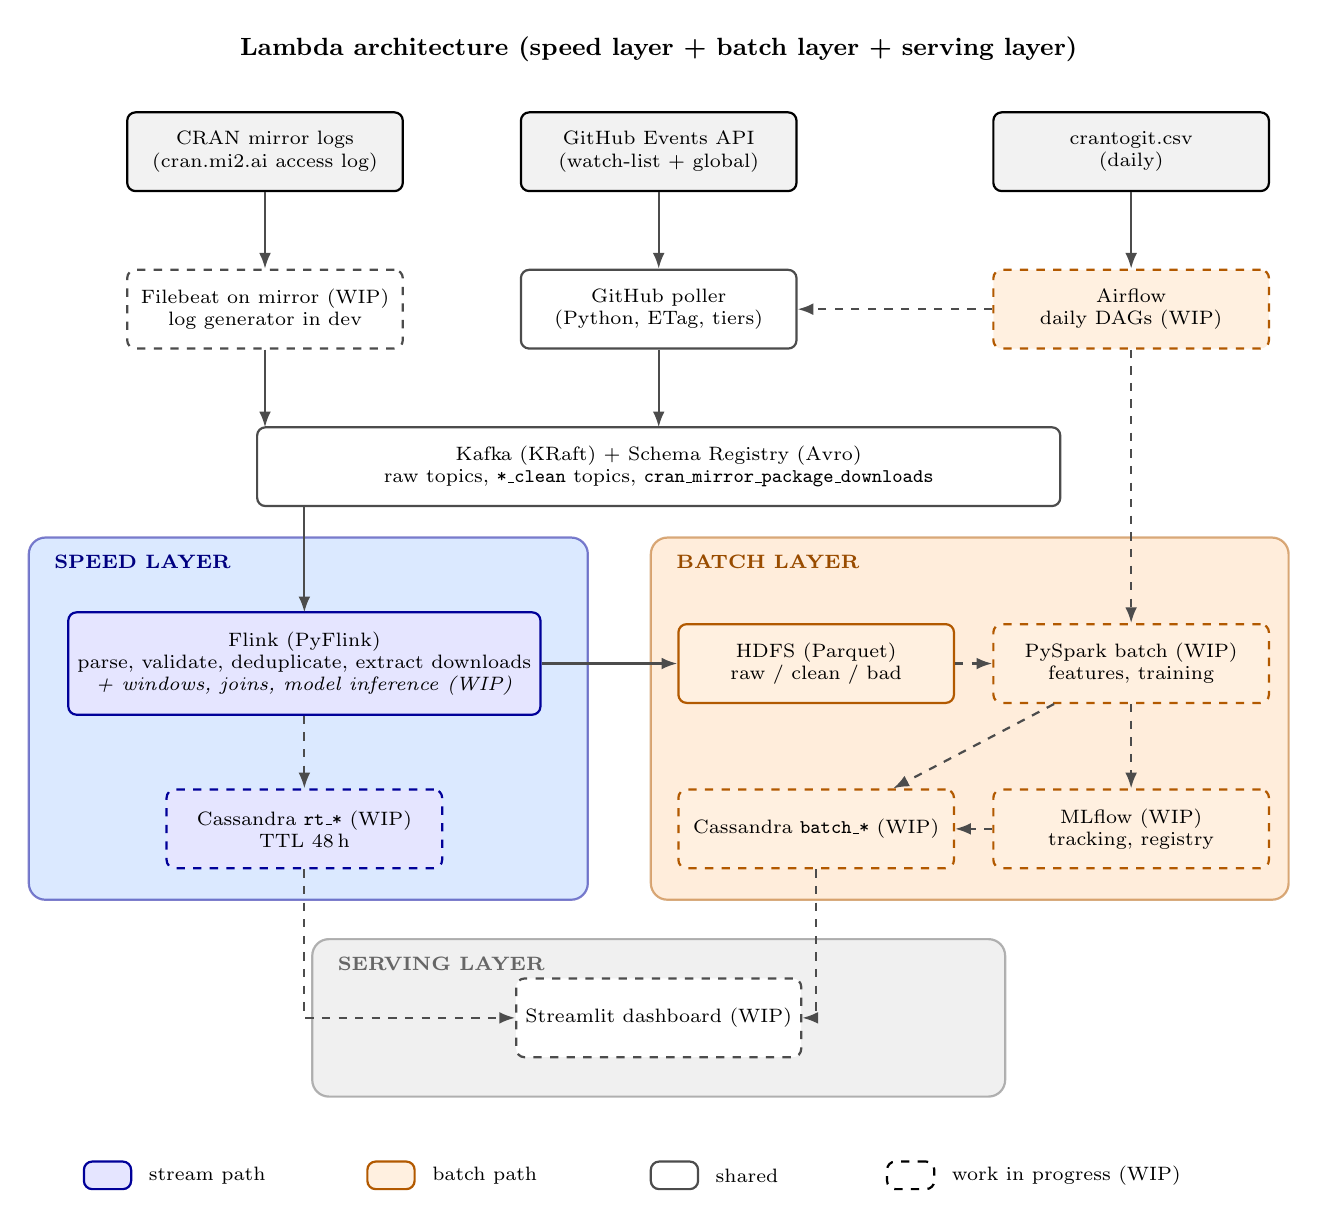
\begin{tikzpicture}[x=1cm,y=1cm,
  box/.style={draw,rounded corners=3pt,minimum width=3.5cm,minimum height=1.0cm,align=center,font=\scriptsize,thick},
  src/.style={box,fill=gray!10},
  stream/.style={box,fill=blue!10,draw=blue!60!black},
  batch/.style={box,fill=orange!12,draw=orange!70!black},
  shared/.style={box,fill=white,draw=black!70},
  plan/.style={dashed},
  flow/.style={-{Latex[length=2mm]},thick,gray!60!black},
  pflow/.style={-{Latex[length=2mm]},thick,gray!60!black,dashed},
  layer/.style={font=\bfseries\scriptsize,anchor=north west}]
  % ---- translucent layer regions
  \begin{scope}[on background layer]
    \fill[blue!60!cyan,opacity=0.14,rounded corners=6pt] (0.0,-4.9) rectangle (7.1,-9.5);
    \draw[blue!60!black,opacity=0.5,rounded corners=6pt,thick] (0.0,-4.9) rectangle (7.1,-9.5);
    \fill[orange,opacity=0.14,rounded corners=6pt] (7.9,-4.9) rectangle (16.0,-9.5);
    \draw[orange!70!black,opacity=0.5,rounded corners=6pt,thick] (7.9,-4.9) rectangle (16.0,-9.5);
    \fill[gray,opacity=0.12,rounded corners=6pt] (3.6,-10.0) rectangle (12.4,-12.0);
    \draw[gray,opacity=0.6,rounded corners=6pt,thick] (3.6,-10.0) rectangle (12.4,-12.0);
  \end{scope}
  \node[layer,text=blue!50!black] at (0.2,-5.0) {SPEED LAYER};
  \node[layer,text=orange!60!black] at (8.1,-5.0) {BATCH LAYER};
  \node[layer,text=black!60] at (3.8,-10.1) {SERVING LAYER};
  \node[font=\bfseries\small] at (8,1.3) {Lambda architecture (speed layer + batch layer + serving layer)};
  % ---- sources and ingestion
  \node[src] (logs) at (3,0) {CRAN mirror logs\\(cran.mi2.ai access log)};
  \node[src] (gh)   at (8,0) {GitHub Events API\\(watch-list + global)};
  \node[src] (ctg)  at (14,0) {crantogit.csv\\(daily)};
  \node[shared,plan] (prod) at (3,-2) {Filebeat on mirror (WIP)\\log generator in dev};
  \node[shared] (poll) at (8,-2) {GitHub poller\\(Python, ETag, tiers)};
  \node[batch,plan] (af) at (14,-2) {Airflow\\daily DAGs (WIP)};
  \node[shared,minimum width=10.2cm] (kafka) at (8,-4) {Kafka (KRaft) + Schema Registry (Avro)\\raw topics, \texttt{*\_clean} topics, \texttt{cran\_mirror\_package\_downloads}};
  % ---- speed layer
  \node[stream,minimum width=5.8cm,minimum height=1.3cm] (flink) at (3.5,-6.5) {Flink (PyFlink)\\parse, validate, deduplicate, extract downloads\\\textit{+ windows, joins, model inference (WIP)}};
  \node[stream,plan] (rt) at (3.5,-8.6) {Cassandra \texttt{rt\_*} (WIP)\\TTL 48\,h};
  % ---- batch layer
  \node[batch] (hdfs) at (10,-6.5) {HDFS (Parquet)\\raw / clean / bad};
  \node[batch,plan] (spark) at (14,-6.5) {PySpark batch (WIP)\\features, training};
  \node[batch,plan] (bt) at (10,-8.6) {Cassandra \texttt{batch\_*} (WIP)};
  \node[batch,plan] (mlf) at (14,-8.6) {MLflow (WIP)\\tracking, registry};
  % ---- serving
  \node[shared,plan] (st) at (8,-11.0) {Streamlit dashboard (WIP)};
  % ---- flows
  \draw[flow] (logs) -- (prod);
  \draw[flow] (gh) -- (poll);
  \draw[flow] (ctg) -- (af);
  \draw[flow] (prod) -- (3,-3.5);
  \draw[flow] (poll) -- (8,-3.5);
  \draw[pflow] (af) -- (poll);
  \draw[flow] (3.5,-4.5) -- (3.5,-5.85);
  \draw[flow] (flink.east) -- (hdfs.west);
  \draw[pflow] (flink) -- (rt);
  \draw[pflow] (hdfs) -- (spark);
  \draw[pflow] (af) -- (spark.north);
  \draw[pflow] (spark) -- (mlf);
  \draw[pflow] (spark) -- (bt);
  \draw[pflow] (mlf) -- (bt);
  \draw[pflow] (rt.south) |- (st.west);
  \draw[pflow] (bt.south) |- (st.east);
  % ---- legend
  \node[stream,minimum width=0.6cm,minimum height=0.35cm] at (1,-13.0) {};
  \node[anchor=west,font=\scriptsize] at (1.4,-13.0) {stream path};
  \node[batch,minimum width=0.6cm,minimum height=0.35cm] at (4.6,-13.0) {};
  \node[anchor=west,font=\scriptsize] at (5.0,-13.0) {batch path};
  \node[shared,minimum width=0.6cm,minimum height=0.35cm] at (8.2,-13.0) {};
  \node[anchor=west,font=\scriptsize] at (8.6,-13.0) {shared};
  \node[box,dashed,minimum width=0.6cm,minimum height=0.35cm] at (11.2,-13.0) {};
  \node[anchor=west,font=\scriptsize] at (11.6,-13.0) {work in progress (WIP)};
\end{tikzpicture}}
\caption{Solution architecture -- \textbf{Lambda architecture} (speed layer in blue, batch layer in orange,
serving layer in grey, shared components in white; dashed = work in progress).}
\label{fig:arch}
\end{figure}

\subsection{Data flows}

\begin{enumerate}
  \item \textbf{CRAN logs:} mirror access log $\to$ Filebeat (generator in dev) $\to$ \texttt{cran\_\allowbreak{}mirror\_\allowbreak{}logs} $\to$ Flink ingest $\to$ \texttt{cran\_\allowbreak{}mirror\_\allowbreak{}logs\_\allowbreak{}clean} + HDFS
        (raw, clean, bad) $\to$ Flink download extraction $\to$ \texttt{cran\_\allowbreak{}mirror\_\allowbreak{}package\_\allowbreak{}downloads} + HDFS.
  \item \textbf{GitHub:} crantogit $\to$ watch-list $\to$ poller $\to$ \texttt{github\_\allowbreak{}repo\_\allowbreak{}updates} (+ \texttt{github\_\allowbreak{}repo\_\allowbreak{}list}) $\to$
        Flink ingest $\to$ \texttt{github\_\allowbreak{}repo\_\allowbreak{}updates\_\allowbreak{}clean} + HDFS.
  \item \textbf{Speed path} \planned: clean topics $\to$ Flink windows and joins (and model inference) $\to$ Cassandra \texttt{rt\_\allowbreak{}*} $\to$ Streamlit.
  \item \textbf{Batch path} \planned: HDFS Parquet $\to$ PySpark (scheduled by Airflow) $\to$ features and forecasts $\to$ MLflow and Cassandra \texttt{batch\_\allowbreak{}*} $\to$ Streamlit.
\end{enumerate}

\subsection{Technologies and tools}

\begin{table}[H]
\centering
\caption{All technologies, implemented and planned.}
\small
\begin{tabularx}{\textwidth}{@{}L{2.9cm}L{3.6cm}L{2.7cm}Y@{}}
\toprule
\textbf{Layer} & \textbf{Technology} & \textbf{Status} & \textbf{Role} \\
\midrule
Ingestion & GitHub poller & \done & Acquire GitHub events and publish them to Kafka \\ Log shipping & Filebeat (log generator in dev) & \planned & Ship the mirror access log to Kafka \\
Messaging & Kafka 4.3.2 (KRaft), Schema Registry 8.4.1 & \done & Buffering, replay, Avro schema governance \\
Stream processing & Flink 1.20.3 (PyFlink, Table API/SQL) & \partialimpl & Validation, deduplication, extraction; later windows/joins \\
Batch storage & HDFS 3.4.2, Parquet & \done & Immutable raw and clean history \\
Batch processing & Spark (PySpark) & \planned & Aggregates, features, training \\
Orchestration & Airflow 3.4.0 (Postgres metadata DB) & \partialimpl & Scheduling of batch jobs and watch-list refresh \\
Serving storage & Cassandra 5.0.9 & \partialimpl & \texttt{rt\_\allowbreak{}*} (TTL) and \texttt{batch\_\allowbreak{}*} tables \\
ML & MLflow & \planned & Experiment tracking and model registry \\
Visualisation & Streamlit & \planned & Dashboard \\
Deployment & Docker Compose (dev / stage / prod env files), stage and prod VMs on the mirror's network & \done & Reproducible environments, init scripts \\
\bottomrule
\end{tabularx}
\end{table}

\subsection{Deployment environments}

The system runs in three environments, all deployed with Docker Compose from the same \texttt{docker-compose.yml}; only the
environment file (\texttt{deploy/stage.env}, \texttt{deploy/prod.env}) differs. Stage and prod are two identical virtual machines on the
same network as the CRAN mirror, each with a static IP address.

\begin{table}[H]
\centering
\caption{Deployment environments.}
\small
\begin{tabularx}{\textwidth}{@{}L{2.4cm}L{4.2cm}L{3.2cm}Y@{}}
\toprule
\textbf{Environment} & \textbf{Host} & \textbf{Storage} & \textbf{Notes} \\
\midrule
Dev & Developer machines & Docker named volumes & One HDFS DataNode; log generator and GitHub poller started on demand (\texttt{deploy/up.sh}) \\
Stage & VM, 16 cores, 64\,GB RAM, static IP, same network as the mirror & 100\,GB SSD, 1\,TB HDD; bind mounts under \texttt{/srv/bigdata/} & Three HDFS DataNodes, replication~2 (\texttt{COMPOSE\_PROFILES=ha}); \texttt{deploy/stage.env} \\
Prod & VM, 16 cores, 64\,GB RAM, static IP, same network as the mirror & 100\,GB SSD, 1\,TB HDD; bind mounts under \texttt{/srv/bigdata/} & As stage; Airflow secrets in an untracked \texttt{prod.secrets.env}; \texttt{deploy/prod.env} \\
\bottomrule
\end{tabularx}
\end{table}

\begin{itemize}
  \item \textbf{Access:} both VMs are reached over SSH through a bastion host, so they are not directly reachable from outside.
  \item \textbf{Network:} services are published only on the VM's static address (\texttt{BIND\_ADDRESS}), and Kafka advertises it to
        external clients (\texttt{KAFKA\_EXTERNAL\_HOST}).
  \item \textbf{Deployment:} Docker Compose; \texttt{deploy/init.sh} creates the Kafka topics, registers the Avro schemas, creates the HDFS
        directories and the Cassandra keyspace.
  \item \textbf{Disk layout:} the 100\,GB SSD holds the operating system, Docker images, Kafka, Cassandra, the Airflow metadata
        database and the HDFS NameNode metadata (latency-sensitive, small). The 1\,TB HDD holds the HDFS DataNode blocks, i.e.\ the
        growing raw and clean history, which is written and read sequentially. Every data path is an environment variable
        (\texttt{KAFKA\_DATA\_DIR}, \texttt{CASSANDRA\_DATA\_DIR}, \texttt{HDFS\_DATANODE*\_DIR}, \ldots), so if the SSD turns out too small a component can be moved to the HDD by
        changing the env file only.
\end{itemize}

Being on the mirror's network means that Filebeat on the mirror can produce log lines to Kafka over the internal network, without
exposing the broker to the internet, and the static addresses give clients a stable bootstrap address. The three HDFS DataNodes of the
\texttt{ha} profile run on one VM, so replication~2 protects against the loss of a DataNode container or its disk, but not against the loss of the VM.

% =====================================================================
\section{Analytical Approach}\label{sec:analytics}
% =====================================================================

\begin{table}[H]
\centering
\caption{Planned analytical tasks.}
\small
\begin{tabularx}{\textwidth}{@{}L{2.5cm}L{2.2cm}L{2.2cm}L{3.0cm}Y@{}}
\toprule
\textbf{Task} & \textbf{Type} & \textbf{Mode} & \textbf{Method (candidate)} & \textbf{Presentation} \\
\midrule
A. Hourly load forecast (7\,d) & Regression / time series & Batch training, daily forecast & Gradient boosting on lag features; seasonal baseline & Forecast curve with confidence band; maintenance-window suggestion \\
B. Bot / CI detection & Classification & Batch training; stream inference & Random forest / gradient boosting on session features; rule-based baseline & Share of bot traffic over time; list of flagged clients \\
C. Release-to-download lag & Statistical analysis & Batch & Peak detection on hourly series after the release timestamp & Per-package lag chart, version migration curves \\
D. Surge detection & Anomaly detection & Stream & Windowed count vs.\ rolling baseline (Flink) & Real-time alerts \\
E. Top packages and error rates & Descriptive aggregation & Stream (windows) + batch (history) & Sliding/tumbling windows; daily Spark aggregates & Live top-$N$ table, error rate, velocity \\
F. Package activity segmentation & Clustering (optional) & Batch & $k$-means on download and release features & Active vs.\ dormant packages \\
\bottomrule
\end{tabularx}
\end{table}

\hd{Batch vs.\ stream.} Everything that must react within seconds (top packages, surge alerts, error rate, bot inference with a loaded model)
runs in Flink and writes to \texttt{rt\_\allowbreak{}*} tables with TTL. Everything needing long history (model training, forecasts, adoption curves)
runs in Spark over HDFS Parquet, scheduled daily by Airflow, and writes to \texttt{batch\_\allowbreak{}*}. Models are trained in Spark, registered in MLflow
and loaded by Flink for inference.

\hd{Presentation to end users.} A Streamlit application with three views matching the deliverables of PM1:
(1)~real-time demand (live tables and charts from \texttt{rt\_\allowbreak{}*}), (2)~version adoption and lag (curves from \texttt{batch\_\allowbreak{}*}),
(3)~mirror health (errors, bot share, active/dormant packages, load forecast). Rendering of real-time and historical data in one chart
merges both Cassandra views.

% =====================================================================
\section{Testing}
% =====================================================================

The test documentation is delivered as a separate file (\texttt{\teamname\_\allowbreak{}Tests.pdf}), see \texttt{Milestone\_\allowbreak{}2\_\allowbreak{}Tests.tex}.
Summary of the scope: functional tests of the acquisition modules (poller: ETag handling, rate limits, scheduling,
Kafka sink, watch-list), functional tests of the pre-processing modules (Flink validation, deduplication, extraction), and quality tests of the
transformations (schema conformance, reject-rate, duplicate-free output, partitioning).

% =====================================================================
\section{Project Description from Milestone 1 (unchanged)}\label{sec:pm1}
% =====================================================================

\subsection{Description}
The CRAN Mirror Demand \& Release Pulse Analysis System is an end-to-end Big Data analytics platform engineered to track, analyze, and
correlate software downloads from Poland's primary Comprehensive R Archive Network mirror (cran.mi2.ai) with upstream open-source
development lifecycles across GitHub. By continuously processing web server access logs and GitHub event feeds, the platform bridges the gap
between open-source code commits and real-world package adoption across the Polish data science ecosystem.

The system connects R package artifacts with upstream Git source code using the canonical r-universe crantogit mapping repository,
encompassing over 18,000 R packages. This facilitates unified real-time traffic monitoring and multi-year historical trend modeling.

\subsection{Purpose, target users, key benefits}
\begin{itemize}
  \item \textbf{Purpose:} Correlate real-time download events in Poland with upstream GitHub tags and releases, predicting mirror traffic
        pressure and measuring software adoption velocity.
  \item \textbf{Target users:} the mirror operator (MI2.ai), R package maintainers, and analysts of the Polish R ecosystem.
  \item \textbf{Key benefits:} the operator sees load and unusual traffic (bots, CI runners) as it happens; maintainers see how quickly
        a release is picked up in Poland.
\end{itemize}

\subsection{High-level deliverables from the user's perspective}
\begin{enumerate}
  \item \textbf{Real-time demand dashboard:} live Streamlit interface showing top-downloaded R packages across Poland, request velocity,
        and real-time alerts when new releases trigger download surges.
  \item \textbf{Version adoption \& lag analytics:} time-series reports measuring the elapsed lag between a GitHub release tag and peak mirror
        downloads, including version migration curves.
  \item \textbf{Mirror health view:} HTTP errors (404, 5xx), traffic volume per package, share of bot and CI traffic, and active vs.\ dormant
        packages based on GitHub activity.
\end{enumerate}

\subsection{Core business process}
Three actors: the R package maintainer / developer (tags versions, uploads archives to CRAN, consumes adoption analytics); the CRAN operations /
mirror admin (monitors health, plans capacity and maintenance); and the Big Data analytics engine (streams logs and events, correlates packages
via crantogit, maintains rolling aggregations, serves reconciled views).

\begin{figure}[H]
\centering
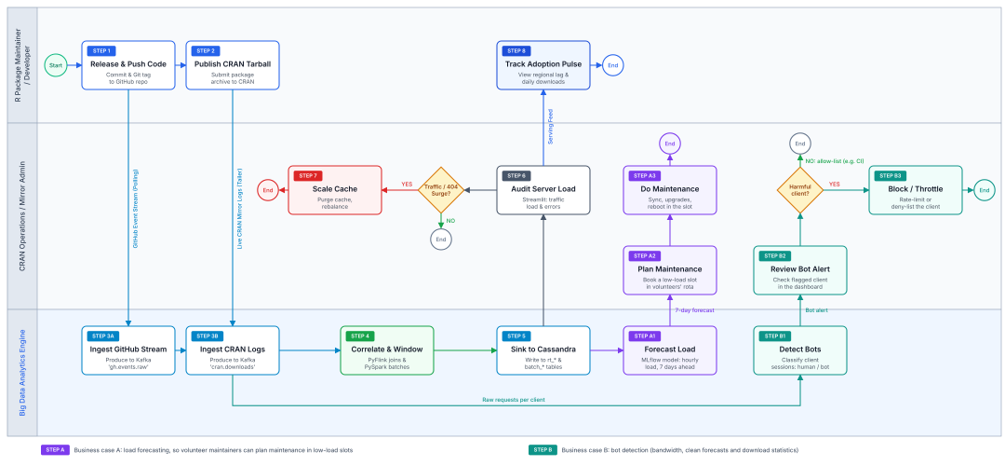
\includegraphics[width=\textwidth]{figures/fig_business_process.png}
\caption{Business process swimlane diagram (from Milestone 1).}
\end{figure}

\subsection{Team members and task allocation}
Unchanged from Milestone 1 (R -- responsible, S -- supporting); see the Milestone 1 report. \todo{Update the allocation table if the actual split of work changed, and add one for the Milestone 2 tasks (report, tests).}

\subsection{Use of GenAI tools}
Generative AI tools are used to research data sources, draft project documentation and diagrams, and generate code. Each AI-assisted task follows the
same workflow: the responsible member writes a prompt with the task requirements and source materials, checks the output against the primary source
and iterates when necessary. Conversations that produced part of the solution are stored in the repository (\texttt{conversations/}).

% =====================================================================
\section{References}
% =====================================================================
\begin{enumerate}
  \item CRAN mirror logs: Polish CRAN mirror access logs (cran.mi2.ai), Warsaw, Poland. Apache common log format.
  \item crantogit dataset: R-Universe CRAN-to-GitHub mapping, \url{https://github.com/r-universe-org/cran-to-git/blob/master/crantogit.csv}
  \item GitHub REST API, Events: \url{https://docs.github.com/en/rest/activity/events}
  \item Official documentation: Apache Kafka (KRaft), Confluent Schema Registry, Apache Flink, Apache Spark, Apache Airflow, Apache Cassandra, Apache Hadoop (HDFS), MLflow, Streamlit.
  \item Source code repository: \url{https://github.com/nizwant/big_data_analytics}
\end{enumerate}

\end{document}
